\section{Wzroce projektowe (3) - czynnościowe }
\subsection{Polecenie (ang. command)}
Polecenie umożliwia zamianę żądania w samodzielny, osobny obiekt. Z tym wzorcem można się spotkać w~kontekście interfejsów użytkownika. Do przycisku może być przypisana akcja (obiekt implementujący interfejs \texttt{ICommand}). Obiekt przycisku powinien posiadać pole/właściwość typu \texttt{ICommand}, można ją przekazać np. jako argument konstruktora. Po kliknięciu w element, instancja przycisku nie jest świadoma akcji, która powinna się wykonać. Pozwala to na łatwą zmianę działania przycisku i umożliwia zachowanie zasady pojedynczej odpowiedzialności (komponent odpowiedzialny za interfejs graficzny nie jest świadomy działania pozostałych warstw aplikacji). Chcąc wprowadzić nową funkcjonalność wystarczy stworzyć nowy obiekt implementujący \texttt{ICommand} i przekazać go do nadawcy (utrzymana jest tym samym zasada otwarte/zamknięte). 

Co więcej, wykorzystanie wzorca Polecenie pozwala na przypisanie kilku przyciskom tej samej czynności. Na przykład operacja zapisywania może być dostępna zarówno jako osobny przycisk jak i~kombinacja klawiszy \texttt{Ctrl+S}.

Dodatkowo omawiany wzorzec pozwala na implementacje cofania, ponawiania operacji oraz ich kolejkowania. Możliwe jest również łączenie wielu prostych poleceń w jedno bardziej skomplikowane.

Jeśli obiekt polecenia do wykonania żądania wymaga dodatkowych parametrów (np. z pól formularza), należy je przekazać jako argument konstruktora (jeśli obiekt ma być niezmienny) albo przez jego właściwości.


%Innym podejściem mogłoby być stworzenie wielu klas dziedziczących po klasie Button np. OkButton, CancelButton, ApplyButton itp...

%Warto zwrócić uwagę na wzorzec MVVM i jak Microsoft podszedł do tematu obłsugi przycisków UI


%PRZYKŁAD Z REFACTORING GURU: Podczas długiego spaceru po mieście, docierasz do miłej restauracji i siadasz przy oknie. Przyjazny kelner szybko przyjmuje zamówienie, spisując je na małym kawałku papieru. Następnie kelner idzie do kuchni i przykleja kartkę na ścianie. Po jakimś czasie zamówienie dociera do szefa kuchni, który przygotowuje danie, a następnie umieszcza posiłek na tacce wraz z zamówieniem. Kelner znajduje tackę, sprawdza zgodność z zamówieniem i zanosi ją do stolika. Zamówienie na papierze stanowi polecenie. Trafia do kolejki, do momentu aż szef kuchni je przygotuje. Zamówienie zawiera wszystkie niezbędne informacje wymagane do przygotowania posiłku. Umożliwia to kucharzowi rozpoczęcie gotowania od razu, zamiast ustalać szczegóły z klientem na własną rękę.


\begin{figure}[hbt!]
	\centering
	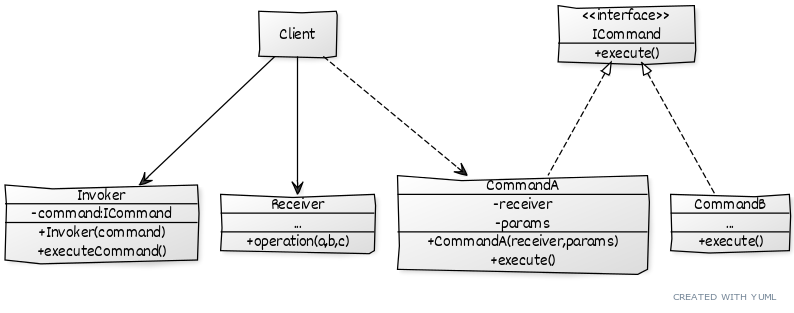
\includegraphics[width=0.9\linewidth]{images/CommandUml}
	\caption{Diagram UML wzorca Polecenie.}
	\label{lab4/fig/CommandUml}
\end{figure}
%[Client]->[Invoker]
%[Client]->[Receiver]
%[Client]-.->[CommandA]
%[ICommand]^-.-[CommandA]
%[ICommand]^-.-[CommandB]
%
%[Client]
%[Invoker|-command:ICommand|+Invoker(command);+executeCommand()]
%[≪interface≫;ICommand|+execute();]
%[CommandA|-receiver;-params|+CommandA(receiver,params);+execute()]
%[CommandB|...|+execute()]
%[Receiver|...|+operation(a,b,c)]

\subsubsection{Zadanie 1}
Utwórz projekt aplikacji konsolowej .NET 5.0. W nowym pliku dodaj interfejs \texttt{ICommand} z dwiema deklaracjami metod: \texttt{void Execute()} oraz \texttt{void Undo()}.

Dodaj klasę \texttt{Character} z jedną publiczną właściwością typu \texttt{Vector3} o nazwie \texttt{Position} (konieczne będzie dodanie przestrzeni nazw \texttt{using System.Numerics}):
\begin{lstlisting}
public class Character
{
	public Vector3 Position { get; set; }
}
\end{lstlisting}

Następnie do projektu dodaj klasę o nazwie \texttt{Move} implementującą interfejs \texttt{ICommand}. Niech posiada ona konstruktor z trzema parametrami, określającymi obiekt do przesunięcia, wektor o jaki ma zostać przesunięty obiekt oraz długość przesunięcia (domyślnie równą jeden):
\begin{lstlisting}
public class Move : ICommand
{
	private readonly Character objectToMove;
	private readonly Vector3 direction;
	private readonly float distance;
	
	public Move(Character objectToMove, Vector3 direction, float distance = 1f)
	{
		this.objectToMove = objectToMove;
		this.direction = direction;
		this.distance = distance;
	}

	//...
\end{lstlisting}
Aby skorzystać ze struktury \texttt{Vector3} również konieczne jest dodanie przestrzeni nazw \texttt{System.Numerics} w~tej klasie. Zaimplementuj w~\texttt{Move} interfejs, tak aby po wywołaniu metody \texttt{Execute()} pozycja przekazanego w konstruktorze obiektu została zaktualizowana o wektor \texttt{direction} (również przekazany jako argument konstruktora) np. w następujący sposób:
\begin{lstlisting}
public class Move : ICommand
{
	//...	
	public void Execute() => objectToMove.Position += direction * distance;
	//...
}
\end{lstlisting}
Analogicznie zaimplementuj operację \texttt{Undo()}.

Wzorzec Polecenie często jest wykorzystywany do przechowywania, cofania i ponawiania jakieś operacji. Dodaj do projektu klasę \texttt{CommandHandler}, która będzie odpowiedzialna za przechowywanie poleceń i~umożliwiała ich cofanie oraz ponowne wywoływanie:
\begin{lstlisting}
public class CommandHandler
{
	private readonly Stack<ICommand> commands = new();
	private readonly Stack<ICommand> redos = new();
	
	public void Add(ICommand command){}
	public void Undo(){}
	public void Redo(){}
}
\end{lstlisting}
Zaimplementuj metody: \texttt{Add}, \texttt{Undo} oraz \texttt{Redo}.

Następnie w klasie \texttt{Character} dodaj prywatne pole typu \texttt{CommandHandler}. Dodatkowo umieść w~niej metody \texttt{Move}, \texttt{Undo} oraz \texttt{Redo}. Będą one obsługiwać operacje ,,przesuwania'' obiektu typu \texttt{Character} wykorzystując \texttt{CommandHandler}.
\begin{lstlisting}
public class Character
{
	public Vector3 Position { get; set; }
	private readonly CommandHandler commands = new();
	
	public void Move(ICommand command)
	{
		commands.Add(command);
		this.PrintPosition();
	}
	
	public void Undo()
	{
		//...
	}
	
	public void Redo()
	{
		//...
	}
	
	private void PrintPosition() => Console.WriteLine(\$"Current position: {this.Position}");
}
\end{lstlisting}
Dodaj implementację metod \texttt{Undo} oraz \texttt{Redo}.

W metodzie \texttt{Main} dodaj obiekt typu \texttt{Character} i cztery obiekty typu \texttt{Move}, następnie wywołując metody \texttt{Move}, \texttt{Undo} i \texttt{Redo} zbadaj poprawność napisanych klas:
\begin{lstlisting}
class Program
{
	static void Main(string[] args)
	{
		var character = new Character();
		ICommand left = new Move(character, new Vector3(-1f,0f,0f), 1f);
		ICommand right = new Move(character, new Vector3(1f, 0f, 0f), 1f);
		ICommand up = new Move(character, new Vector3(0f, 1f, 0f), 1f);
		ICommand down = new Move(character, new Vector3(0f, -1f, 0f), 1f);
		
		character.Move(left);
		character.Move(up);
		character.Move(up);
		character.Undo();
		character.Redo();
	}
}
\end{lstlisting}

\subsection{Strategia (ang. strategy)}

Klient, aby zrealizować pewne zadania może wykorzystywać konkretny algorytm. Często może się on zmieniać w~czasie albo być zależny od dodatkowych czynników np. wyboru opcji przez użytkownika programu. Wzorzec Strategia pozwala utworzyć rodzinę algorytmów realizujących dane zadanie w różny sposób. Dalej za pomocą konstruktora, właściwości albo metody klient może podmienić obiekt strategii i tym samym zmienić sposób realizacji danej czynności przez daną klasę. Gorszą alternatywą mogłoby być zbudowanie na stałe wielu algorytmów w daną klasę i naruszenie tym samym pierwszych dwóch zasad \textbf{SO}LID (\ref{lab1/sec/srpPrinciple} i \ref{lab1/sec/ocpPrinciple}).

Strategia bazuje na mechanizmie odwracania zależności. Koncepcyjnie DI jest raczej zarezerwowane dla przypadków, gdzie podczas wykonywania się programu dane zachowanie (wstrzykiwany obiekt) jest stałe. Jeśli natomiast zakładamy, że sposób realizacji danego algorytmu będzie się zmieniał to wtedy odnosimy się raczej do wzorca Strategia. Różnice między nimi są niewielkie i subtelne. Pod względem struktury strategia jest podobna również do mostu i stanu, które też bazują na kompozycji. Mimo, że pod względem struktury są ona do siebie bardzo podobne, nazewnictwo stosowane w tych wzorcach powinno programistę informować o~specyficznym problemie, który został za jego pomocą rozwiązany.

W programowaniu obiektowym istnieje zasada, aby przekładać kompozycję nad dziedziczeniem. Podobnym do strategii wzorcem jest również Metoda Szablonowa wykorzystująca dziedziczenie. Takie podejście sprawia, że strategia jest na sztywno połączona z~klasa \texttt{Context}, nie możliwe jest dynamiczne zmienianie algorytmu. Dodatkowo utrudnia to zrozumienie kodu. 

%Refactoring guru
%Polecenie i Strategia mogą wydawać się podobne, ponieważ oba mogą służyć parametryzacji obiektu jakimś działaniem. Mają jednak inne cele. Za pomocą Polecenia można konwertować dowolne działanie na obiekt. Parametry działania stają się polami tego obiektu. Konwersja zaś pozwala odroczyć wykonanie działania, kolejkować je i przechowywać historię wykonanych działań, a także wysyłać polecenia zdalnym usługom, itd. Z drugiej strony, Strategia zazwyczaj opisuje różne sposoby wykonywania danej czynności, pozwalając zamieniać algorytmy w ramach jednej klasy kontekstu.

Diagram UML omawianego wzorca został przedstawiony na diagramie UML~\ref{lab4/fig/StrategyUml}. Klient tworzy obiekt konkretnej strategi (musi ona implementować wspólny dla wszystkich strategi interfejs). Dalej taka instancja może zostać przekazana np. przy wykorzystaniu metody (\texttt{setStrategy(strategy)}) do obiektu realizującego daną czynność. Klient ma możliwość w trakcie działania programu płynnie zmieniać sposób realizowania danej czynności.

\begin{figure}[hbt!]
	\centering
	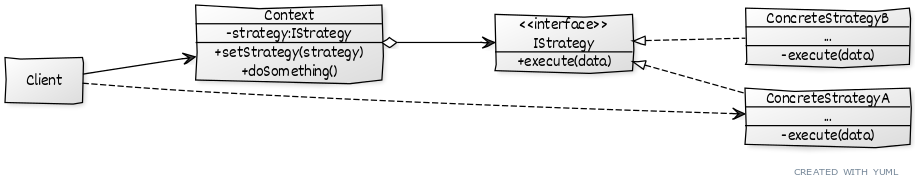
\includegraphics[width=0.9\linewidth]{images/StrategyUml}
	\caption{Diagram UML wzorca Strategia.}
	\label{lab4/fig/StrategyUml}
\end{figure}
%[Client]->[Context]
%[Client]-.->[ConcreteStrategyA]
%[Context]<>->[IStrategy]
%[IStrategy]^-.-[ConcreteStrategyA]
%[IStrategy]^-.-[ConcreteStrategyB]
%
%[Client]
%[Context|-strategy:IStrategy|+setStrategy(strategy);+doSomething()]
%[≪interface≫;IStrategy|+execute(data);]
%[ConcreteStrategyA|...|-execute(data)]
%[ConcreteStrategyB|...|-execute(data)]

%Użycie wzorca strategii powinno być podyktowane faktem, że klasa korzysta z różnych algorytmów do wykonania \textbf{tej samej} czynności. Co więcej, zwykle te algorytmy mogą się zmieniać w czasie. Dodatkowo algorytm ułatwia odizolowanie algorytmu od logiki biznesowej. Pozwala również ukryć szczegóły implementacyjne np. złożone struktury danych. 

Jeżeli obiekt strategi potrzebuje dodatkowych argumentów mogą one zostać udostępnione przez kontekst w~momencie wywoływania algorytmu. Ewentualnie \texttt{Context} może przekazać do obiektu strategii samego siebie.

Przykładem zastosowania wzorca Strategia może być nawigacja i różne algorytmy obliczania optymalnej drogi. Na przykład w~zależności od środka transportu może być stosowany inny obiekt \texttt{ConcreteStrategy}. W~bibliotece \texttt{ObjectWindows} strategia jest stosowana w oknach dialogowych do sprawdzania poprawności wprowadzanych przez użytkownika danych. Zestaw oferuje część predefiniowanych algorytmów, a~użytkownik jeśli nie znajdzie dla niego odpowiedniego, może łatwo rozszerzyć możliwości przez stworzenie własnego obiektu implementującego konkretny interfejs. Strategia może również być wykorzystywana w~algorytmach parsujących (różne algorytmy w zależności od formatu danych wejściowych) albo optymalizacji kompilowanego kodu (inne obiekty dla poszczególnych rodzajów i poziomów kompilacji).

\subsubsection{Zadanie 2}
W solucji dodaj kolejny projekt aplikacji konsolowej .NET 5.0. Dodaj w nim interfejs \texttt{IRouteStrategy} z~jedną metodą \texttt{BuildRoute}, nie przyjmującą żadnych argumentów i~zwracającą typ \texttt{void}. 

Następnie dodaj trzy klasy: \texttt{PublicTransportStrategy}, \texttt{RoadStrategy} i \texttt{WalkingStrategy} implementujące interfejs \texttt{IRouteStrategy} np. w następujący sposób:
\begin{lstlisting}
public class PublicTransportStrategy : IRouteStrategy
{
	public void BuildRoute() => Console.WriteLine("Public transport strategy has been used for travel time estimation.");
}
\end{lstlisting}

Dalej dodaj do projektu klasę \texttt{Navigator} z konstruktorem przyjmującym argument typu \texttt{IRouteStrategy} i przypisującym go do prywatnego pola. 

Dodatkowo w klasie \texttt{Navigator} dodaj dwie metody: \texttt{SetStrategy} oraz \texttt{Navigate}:
\begin{lstlisting}
public class Navigator
{
	//...
	
	public void SetStrategy(IRouteStrategy strategy) => this.routeStrategy = strategy;
	
	public void Navigate() => this.routeStrategy.BuildRoute(); //in real scenario method should return direction, trace from point A to point B
}
\end{lstlisting}

W metodzie \texttt{Main} sprawdź działanie przykładowego programu:
\begin{lstlisting}
static void Main(string[] args)
{
	var context = new Navigator(new RoadStrategy());
	context.Navigate();
	
	context.SetStrategy(new PublicTransportStrategy());
	context.Navigate();
	
	context.SetStrategy(new WalkingStrategy());
	context.Navigate();
}
\end{lstlisting}

Oczywiście metody \texttt{BuildRoute} w~normalnym przypadku powinny przyjmować współrzędne lokalizacyjne i~zwracać faktyczną drogę umożliwiającą przemieszczenie się z~punktu A do punktu B.

\subsection{Mediator (ang. mediator)}

Wzorzec projektowy mediator umożliwia kapsułkowanie interakcji pomiędzy obiektami poprzez dodatkowy obiekt mediatora. Obiekty mogą się komunikować jedynie wykorzystując ten obiekt.

%Analogią może być wieża kontrolerów lotów na lostniku. Piloci nie rozmawiają między sobą nawzajem, a komunikują się przez swego rodzaju moderatora. 

Wyobraźmy sobie sytuację, w której okno dialogowe składa się z wielu widgetów. Pewne pole może być aktywne albo nieaktywne w zależności od wybranej wcześniej opcji widgetu typu \texttt{checkbox}. W innym przypadku przycisk do wysłania formularza aktywowany jest dopiero po wypełnieniu wszystkich niezbędnych pól. Bez użycia obiektu mediatora poszczególne instancje widgetów musiałby posiadać referencje do sobie nawzajem, aby np. po zaznaczeniu pola wyboru, aktywować pole tekstowe. Ponowne użycie takich elementów staje się utrudnione, a czytelność kodu się pogarsza.


Zamiast zmuszać obiekty do posiadania informacji o sobie nawzajem można wprowadzić dodatkowy obiekt moderatora (diagram UML przedstawiono poniżej\ref{lab4/fig/MediatorUml}), który będzie pośredniczył w~komunikacji między obiektami. Komponenty w tej sytuacji są zależne jedynie od obiektu moderatora i to do niego kierują informację np. o zmianie stanu pola wyboru. Na przykład momencie kliknięcia przycisku przez użytkownika obiekt \texttt{Button} mógłby wysyłać informację o~operacji do mediatora, który sprawdzałby pozostałe pola i podejmował decyzję o wysłaniu formularza. 


Obiekty mogą się komunikować np. z~wykorzystaniem zdarzeń albo wzorca obserwatora. We wzorcu MVC (ang. Model View Controller - Model Widok Kontroler) moderatorem jest kontroler.

\begin{figure}[hbt!]
	\centering
	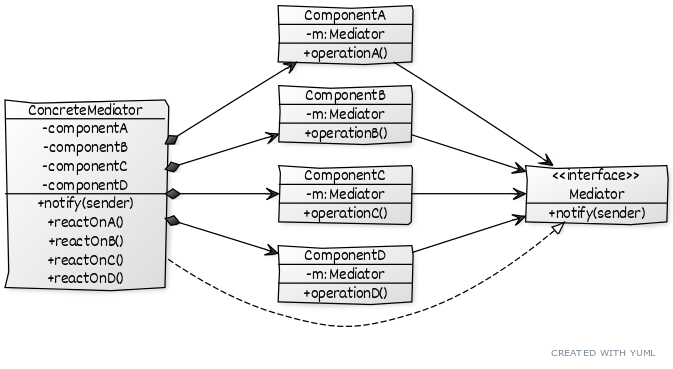
\includegraphics[width=0.9\linewidth]{images/MediatorUml}
	\caption{Diagram UML wzorca Mediator.}
	\label{lab4/fig/MediatorUml}
\end{figure}
%[ConcreteMediator]++->[ComponentA]
%[ConcreteMediator]++->[ComponentB]
%[ConcreteMediator]++->[ComponentC]
%[ConcreteMediator]++->[ComponentD]
%[Mediator]^-.-[ConcreteMediator]
%[ComponentA]->[Mediator]
%[ComponentB]->[Mediator]
%[ComponentC]->[Mediator]
%[ComponentD]->[Mediator]
%
%[≪interface≫;Mediator|+notify(sender)]
%[ConcreteMediator|-componentA;-componentB;-componentC;-componentD|+notify(sender);+reactOnA();+reactOnB();+reactOnC();+reactOnD()]
%[ComponentA|-m: Mediator|+operationA()]
%[ComponentB|-m: Mediator|+operationB()]
%[ComponentC|-m: Mediator|+operationC()]
%[ComponentD|-m: Mediator|+operationD()]

Wzorzec Mediator warto zastosować jeśli istnieje wiele zależności pomiędzy klasami, a ich ponowne użycie w~innym programie jest z tego powodu mocno utrudnione. Podobnym wzorcem do Mediatora jest Fasada. Główną różnicą między nimi jest fakt, że ta druga posiada zależności jednokierunkowe. Obiekty reprezentowane przez fasadę mogą kierować żądania do podsystemów, ale podsystemy nie mogą komunikować się z Fasadą.

Wadą omawianego wzorca jest fakt, że mediator z czasem może stać się bardzo złożony tzw. Boski Obiekt. Taki obiekt jest przykładem antywzorca projektowego. Posiada on zazwyczaj wiele zależności i~łamie zasadę pojedynczej odpowiedzialności. Dodatkowo należy szczególnie zaznaczyć, że Mediator powinien być używany w~większych projektach. Wprowadza on dodatkową złożoność. Tak samo jak z większością wzorców projektowych jeśli tworzymy proste aplikacje, albo krótkie przykłady tak jak na laboratoriach to użycie niektórych wzorców jest niepożądane. Nie ma sensu komplikować prostego, małego projektu.
Jeśli jednak aplikacja zaczyna się rozrastać to dobre praktyki i wzorce zaczynają mieć znaczenie. %Trochę jak z huśtawką rozmiar i złożoność aplikacji musimy równoważyć dobrymi wzorcami i zasadami czy liczbą testów. 
Tak samo Madiator jak i opisany w~kolejnych akapitach wzorzec CQRS \textbf{nie są} korzystne dla wszystkich aplikacji.

%\subsubsection{Jason Taylor - CleanArchitecture}
%Solucja powinna być podzielona na odpowiednie komponenty. Nie ma sensu tworzyć ogromnej ilości osobnych zestawów, które mogłyby zostać umieszczone w folderach. Należy natomiast w przemyślany sposób komponenty rozdzielać od siebie tam gdzie jest to przydatne. 
%
%W pierwszej kolejności warto oddzielić kod źródłowy oprogramowania od testów. Można to zrealizować przez stworzenie dwóch osobnych folderów. W pierwszym można umieścić cztery warstwy np.:
%\begin{itemize}
%	\item Application - zawiera logikę związaną w aplikacją. Związana jest z warstwą domeny i niczym więcej. Definiuje ona interfejsy, które powinny być implementowane na przez zewnętrzne warstwy t.j. infrastrukturę oraz WebUI. Jeśli aplikacja wymaga dostępu do serwisu powiadomień, interfejs powinien znaleźć się w warstwie aplikacji, natomiast jego implementacja w infrastrukturze.
%	\item Domain - przechowuje encję, typy wyliczeniowe, wyjątki, interfejsy, typy i logikę specyficzną dla warstwy domeny. Jeśli piszemy projekt związany z finansami to wszystko co ma związek z tą domeną powinno się tam znaleźć. Nie posiada żadnych dodatkowych zależności.
%	\item Infrastructure - zawiera klasy, które pozwalają na dostęp do zewnętrznych zasobów takich jak systemy plików, web serwisy, bazy danych itp. Powinny opierać się na interfejsach zdefiniowanych w warstwie aplikacji.
%	\item WebUI - warstwa prezentacji, odpowiada za interakcję z aplikację. Może to być aplikacja Anuglar, standardowy MVC, Blazor, WPF itp. Opiera się zarówno na warstwie aplikacji oraz infrastruktury. Przy czym należy mieć na uwadze, że powiązanie z warstwą infrastruktury istnieje jedynie, aby umożliwić wstrzykiwanie zależności. Jedynie \texttt{Startup.cs} powinien posiadać referencję do warstwy infrastruktury, w celu rejestracji serwisów.
%\end{itemize}
% Mamy cztery projekty i reprezentują one trzy warstwy. Od środką jest do po kolei domena, infrastruktura, aplikacja oraz WebUI. 
% WebUI jest warstwą prezentacji (najwyższą warstwą), odpowiada za interakcję z aplikacją. Może to być aplikacja Angular, MVC, Blazor, WPF itd.  
% Domain (Entities) np. ToDoItem oraz ToDoList plus osoby folder Exception, Enums, ValueObjects itd. Serce całej aplikacji.
% Application - odpwiada za to jak wykorzystywać encję z domeny. Np. posiada Commands typu. CreateToDoItem, CreateToDoList. Nie zawiera informacji JAK tworzyć te listy, gdzie je przechowywać itd.
% Infrastrature - implementuje abstrakcję z Application.
% WebUI - zależność od warstwy infrastruktury jedynie w celach rejestracji usług.
% Powyższe pozwala nam na czystą i prostą architekturę. 
% W osobnych folderze obok kodu źródłowego należy dodać testy jednostkowe. Osobno można dodać testy akceptacyjne, w innym projekcie związne w warstwą aplikacji i jeszcze w innym te związane z warstwą domeny.
% Jeśli WebUI jest API można go opublikować jako pakiet NuGet, aby innym koledzy z zespołu mogli z niego korzystać. 

\subsubsection{CQRS and MediatR framework}\label{sec/lab4/cqrs}

% Source : https://docs.microsoft.com/en-us/azure/architecture/patterns/cqrs

W prostych aplikacjach webowych często korzysta się z tzw. podejścia CRUD\footnote{Skrót CRUD (ang. Create Read Update Delete) określa cztery podstawowe operacje służące do utrwalania danych np. w bazie danych. Za pomocą tych operacji  np. interfejs użytkownika może dodawać, odczytywać, aktualizować i usuwać rekordy w~bazie danych.}. W sytuacji wielu zapytań o różne obiekty danych (DTO) aplikacja musi wykonywać wiele operacji mapowania. Dodatkowo proces zapisu może wymagać złożonej walidacji i dodatkowej logiki biznesowej. Powoduje to, że model staje się skomplikowany i trudny w utrzymaniu. Mimo tych wad CRUD jest bardzo często (i słusznie) stosowany w prostych aplikacjach. Jeśli domena jest prosta, albo CRUD jest wystarczający nie ma większego sensu stosować omówionego poniżej CQRS.
 
Wraz ze wzrostem złożoności aplikacji mogą pojawiać się dodatkowe problemy. Może okazać się konieczne łączenie wielu rekordów w jeden, albo łączenie kilku rekordów w~jeden wirtualny. W przypadku aktualizacji danych konieczna może być bardziej złożona walidacja danych. 
 
Pewnym rozwiązaniem ułatwiającym skalowanie oraz zapewnienie wysokiej wydajności jest wykorzystanie wzorca CQRS (ang. Command Quary Responsibility Segregation), który oddziela zapytania (Query) i polecenia (Command) do bazy danych. Zapytania \texttt{Queries} nie powinny modyfikować danych, mogą one jedynie czytać dane. Polecenia natomiast służą do dodawania nowych danych, usuwania ich albo aktualizacji. Używany jest inny model do zapisu i odczytu. Pisząc o różnych modelach mamy na myśli różne modele obiektów często działające w różnych procesach, albo na różnych maszynach. Np. w przypadku stron www renderowanie wykorzystuje model zapytań. Jeśli natomiast użytkownik wykona jakąś akcję np. danie kciuka w górę na portalu społecznościowym to takie polecenie jest wysyłane do osobnego modelu do przetworzenia. Innymi korzyściami jest zwiększenie bezpieczeństwa ponieważ ta sama encja nie jest wykorzystywana zarówno do operacji czytania i zapisywania. W przeciwnym przypadku informacje mogłyby zostać użyte w złym kontekście. 

Wykorzystywane modele są elastyczne i łatwe w~utrzymaniu. Skomplikowana logika biznesowa jest zazwyczaj skupiona w modelu zapisu, natomiast odczyt może pozostać względnie prosty. Komponent ten wysyła zazwyczaj jedynie zapytanie do bazy danych oraz serializuje wynik do obiektu DTO. 

CQRS pozwala również na \textbf{fizyczne} oddzielenie danych do czytania i danych do zapisu. Model poleceń może być utrwalany w jednej bazie danych, natomiast model zapytań w drugiej.  W~takich sytuacjach często model zapisu zgłasza zdarzenie za każdym razem, gdy baza danych jest aktualizowana. Baza przechowująca dane do czytania może być taką samą bazą jak ta do zapisu, albo mogą one posiadać zupełnie różne struktury. Takie rozwiązanie pozwala również na sterowanie obciążeniem systemu (zazwyczaj operacje czytania występują częściej niż zapisu). Można również wykorzystać różne struktury, techniki dostępu do danych zoptymalizowane dla zapisu i odczytu. Plusem jest również, że oddzielna część programistów może skupić się na osobnych modelach.

%Polecenia mogą być umieszczane w kolejce i wykonywane asynchronicznie. Nigdy nie powinny one modyfikować bazy danych. Zwracają one DTO, które nie enkapsuluje żadnej wiedzy domenowej. 

Minusem tego wzorca jest wprowadzanie dodatkowej złożoności do programu. Co więcej, jeśli mamy rozdzielone bazy danych dla zapisu i odczytu musimy zapewnić ich spójność.

CQRS jest warto stosować jeśli wiele użytkowników oczekuje równoległego dostępu do danych. Omawiany wzorzec pozwala zminimalizować liczbę konfliktów na poziomie domeny. Dodatkowo jeśli polecenia są skomplikowane, albo trzeba ich wykonać wiele aby zrealizować daną operację np. połączyć dane w obiekt transferu danych (DTO) to model zapisu musi być wstanie obsłużyć wiele poleceń, wykorzystać logikę biznesową oraz walidować wejścia. Operacje te muszą być wykonywane, aby zapewnić poprany stan danych. Im dana dziedzina jest bardziej skomplikowana tym stosowanie CQRS staje się coraz bardziej uzasadnione.

% Nie które implementacje wykorzystują tzw. Event Sourcing pattern. W tym podejściu stan aplikacji jest przechowywany jako sekwencja zdarzeń. Każde zdarzenie reprezentuje zmianę stani danych. Aktualny stan jest konstruowany przez odtwarzanie zdarzeń. Korzyścią jest fakt, że te same zdarzenia mogą być użyte do powiadamiania innych komponentów, w tym modelu odczytu. Model ten może używać zdarzeń to stworzenia migawki aktualnego stanu.


%//Following based on TimCorrey Intro to MediatR
%Front-end API or razor/blazor aplikacja komunikuje się z logiką biznesową i dalej komunikuje się z modułem dostępu do danych i dalej z bazą danych. Mediator wprowadza do tego segmentację, aby usunąć sprzężenia pomiędzy wymienionymi wyżej modułami. 
%
%Mediator otrzymuje nowe żądanie wysłania w naszym przypadku typu \texttt{GetPersonListQuery()}. Mediator szuka wszystkich handlerów, które obsługują dane żądanie. \texttt{GetPersonListHandler} implementował \texttt{IRequestHandler<\textbf{GetPersonListQuaery}, List<PersonModel>>} i to właśnie tego framework MediatR "szuka". Dlatego również konieczne było przekazanie całego zestawu do metody \texttt{service.AddSingleton()}, aby wykorzystując refleksję możliwe było odnalezienie odpowiednich handlerów.
%
%Korzyścią zastosowanie powyższego podejścia jest fakt, że odsunęliśmy logikę pobierania danych od interfejsu użytkownika. Nasza strona nie posiada żadnej prawdziwej logiki. Cała praca odbywa się w handlerach. Co więcej można prosto napisać testy jednostkowe, aby sprawdzić metodę \texttt{Handle}, łatwo można wstrzyknąć obiekt implementujący \texttt{IDataAccess}.


% WebAPI  w ASP.NET wykorzystuje serwisy RESTful. Manipulacja zasobami odbywa się przez żądania POST, GET, PUT oraz DELETE. Do obłsugi żądań API używa kontrolerów, które dziedziczą po \texttt{ControllerBase}. Jeśli chcielibyśmy dodakować obłsugiwać widoki to wtedy możemy dziedziczyć po \texttt{Controller}. Do konfiguracji zachować web API wykorzystywane są atrybuty. Ważne jest, aby kontrolery posiadały sufix \texttt{Controller} inaczej nie będzie można z nich skorzystać, dodatkowo powinny one znajdować się w folderze Controllers. Framework szuka klas, które kończą się tym sufiksem.

% Atrybut [ApiController] dodaje funkcjonalności do kontrolera. //TODO: Doczytać i ogarnąć jakie dokładnie.

\subsubsection{Zadanie 3}
Utwórz dwa nowe projekty w solucji:
\begin{itemize}
	\item ASP.NET Core Web API o nazwe DemoApi (zwróć uwagę, aby zaznaczona była opcja ,,Enable OpenAPI support'')
	\item Class library o nazwie DemoLibrary
\end{itemize}
Oba niech korzystają z .NET 5.0 i domyślnych ustawień projektu.

Zainstaluj \texttt{MediatR.Extensions.Microsoft.DependencyInjection}, jest to pakiet NuGet umożliwiający zarejestrowanie wszystkich handlerów MediatR do kontenera DI. Wraz z nim zainstaluje się również sam pakiet \texttt{MediatR}\footnote{MediatR jest prostą implementacją wzorca Mediator dla .NETu.}.

W folderze Models umieść klasę o nazwie \texttt{PersonModel} o~następujących właściwościach: \texttt{Id} typu \texttt{int}, oraz \texttt{FirstName} i \texttt{LastName} typu \texttt{string}.

Dalej w projekcie DemoLibrary 5 folderów: Commands, DataAccess, Handlers, Models, Queries. W folderze Commands dodaj rekord:
\begin{lstlisting}
public record InsertPersonCommand(string FirstName, string LastName) : IRequest<PersonModel>;
\end{lstlisting}
, a do folderu Queries dodaj dwa rekordy w osobnych dwóch plikach:
\begin{lstlisting}
public record GetPersonByIdQuery(int Id) : IRequest<PersonModel>;
\end{lstlisting}
oraz
\begin{lstlisting}
public record GetPersonListQuery() : IRequest<List<PersonModel>>;
\end{lstlisting}
Interfejsy \texttt{IRequiest<>} pochodzą z dodanego przed chwilą pakietu \texttt{MediatR}. Konieczne będzie dodatnie odpowiedniej przestrzeni nazw.

Dodaj do folderu DataAccess klasę \texttt{DemoDataAccess} implementującą \texttt{IDataAccess}, która będzie źródłem danych:
\begin{lstlisting}
public class DemoDataAccess : IDataAccess
{
	private List<PersonModel> people = new();
	
	public DemoDataAccess()
	{
		people.Add(new PersonModel { Id = 1, FirstName = "Tim", LastName = "Correy" });
		people.Add(new PersonModel { Id = 2, FirstName = "Sue", LastName = "Correy" });
	}
	
	public List<PersonModel> GetPeople() => people;
	public PersonModel InsertPerson(string firstName, string lastName)
	{
		PersonModel p = new() { FirstName = firstName, LastName = lastName };
		p.Id = people.Max(x => x.Id) + 1;
		people.Add(p);
		return p; //return because, client may want to see the new PersonModel with the Id value
	}
}
\end{lstlisting}

Teraz pozostało dodać handlery, zarówno dla poleceń jak i zapytań. W folderze Handlers umieść następujące klasy:
\begin{lstlisting}
public class GetPersonListHandler : IRequestHandler<GetPersonListQuery, List<PersonModel>>
{
	private readonly IDataAccess _data;
	
	public GetPersonListHandler(IDataAccess data) => _data = data;
	public Task<List<PersonModel>> Handle(GetPersonListQuery request, CancellationToken cancellationToken)
	{
		//we have synchro call but we need to return async value.
		//FromResult take synchronous call and turns it into an asynchronous 
		return Task.FromResult(_data.GetPeople());
	}
}
\end{lstlisting}

\begin{lstlisting}
public class GetPersonByIdHandler : IRequestHandler<GetPersonByIdQuery, PersonModel>
{
	private readonly IMediator mediator;
	
	public GetPersonByIdHandler(IMediator mediator) => this.mediator = mediator;
	
	public async Task<PersonModel> Handle(GetPersonByIdQuery request, CancellationToken cancellationToken)
	{
		//database would be much more efficient, one doesn't has to search entirely list for 
		//specific Id
		var results = await mediator.Send(new GetPersonListQuery());
		return results.FirstOrDefault(x => x.Id == request.Id);
	}
}
\end{lstlisting}

\begin{lstlisting}
public class InsertPersonHandler : IRequestHandler<InsertPersonCommand, PersonModel>
{
	private readonly IDataAccess data;
	
	public InsertPersonHandler(IDataAccess data) => this.data = data;
	public Task<PersonModel> Handle(InsertPersonCommand request, CancellationToken cancellationToken)
	{
		return Task.FromResult(data.InsertPerson(request.FirstName, request.LastName));
	}
}
\end{lstlisting}
Pierwsza będzie odpowiedzialna za pobieranie listy wszystkich modeli osób (\texttt{PersonModel}), druga pojedynczego modelu po identyfikatorze \texttt{Id}, trzecia do dodania nowego modelu do ,,bazy danych''.


W projekcie DemoApi dodaj klasę kontrolera do folderu \texttt{Controllers}:
\begin{lstlisting}
[Route("api/[controller]")]
[ApiController]
public class PersonController : ControllerBase
{
	private readonly IMediator mediator;
	
	public PersonController(IMediator _mediator)
	{
		mediator = _mediator;
	}
	
	// GET: api/<PersonController>
	[HttpGet]
	public async Task<List<PersonModel>> Get() //a list
	{
		return await mediator.Send(new GetPersonListQuery());
	}
	
	// GET api/<PersonController>/5
	[HttpGet("{id}")]
	public async Task<PersonModel> Get(int id) //get by id one item
	{
		return await mediator.Send(new GetPersonByIdQuery(id));
	}
	
	// POST api/<PersonController>
	[HttpPost] // insert
	//one liner, very simple controller
	public async Task<PersonModel> Post([FromBody] PersonModel value) =>  await mediator.Send(new InsertPersonCommand(value.FirstName, value.LastName));
	
}
\end{lstlisting}

Na koniec w pliku \texttt{Startup.cs} w metodzie \texttt{ConfigureServices} dodaj do kontenera rejestracje klasy \texttt{IDataAccess} oraz rejestrację wszystkich zależności handlerów i typów mediatora:
\begin{lstlisting}
public void ConfigureServices(IServiceCollection services)
{
	
	/...	
	services.AddSingleton<IDataAccess, DemoDataAccess>();
	services.AddMediatR(System.Reflection.Assembly.Load(nameof(DemoLibrary)));
}
\end{lstlisting}

Po wykonaniu powyższych kroków i uruchomieniu projektu DemoApi powinniśmy móc skorzystać z utworzonego web serwisu wykorzystującego wzorzec mediator oraz CQRS. Skompiluj i uruchom program. Ponieważ podczas tworzenia projektu DemoApi domyślnie została wybrana opcja Enable OpenAPI support, po uruchomieniu projektu otworzony się w oknie przeglądarki internetowej Swagger UI. Pozwoli on na przetestowanie REST API naszej aplikacji.